\section{Descripción del prototipo}
Uno de los objetivos de la realización de este trabajo terminal es permitir al usuario empezar a hacer uso de Big Data de una manera sencilla y sin demasiadas complicaciones. Por lo que se llevo a cabo el desarrollo de un instalador que simplifique el proceso de puesta en marcha del ambiente de análisis de datos.\\
Se trata de una herramienta que asista al usuario en disminuir el número de pasos necesarios para instalar un ambiente que permita llevar a cabo la realización de Big Data sobre de el. 
\\
Podría decirse que la utilidad de este prototipo se refleja al comparar el número de pasos que se enuncian en el manual de instalación de \emph{Luminus}, contra el número de pasos que se siguen al utilizar el instalador mismos que serán comparados dentro de esta sección.\\

\section{Análisis}
La manera en que se pretende que el instalador simplifique el proceso de instalación es automatizando algunas tareas que de otra forma el usuario tendría que realizar una a una, existiendo así la posibilidad de que éste mismo cometa algún error u omita algún paso, y por lo tanto, el ambiente de análisis de datos no pueda ponerse en funcionamiento.\\
Existen diferentes tecnologías para solventar la instalación y configuración de un conjunto previamente determinado de tecnologías, por ejemplo, Docker.\\
Sin embargo, para el uso de Big Data se utilizan tecnologías como Apache Hadoop y Apache Spark, mismas que para estas tecnologías, la instalación y puesta en marcha con Docker se encuentran en fase experimental lo que significa que no es consistente y generaría muchos problemas al momento de querer utilizarlo \cite{dockermalo}.   
\\
Para solventar esto, se decidió hacer uso del Shell Script de Unix/Linux el cual es simplemente un programa que lee los comandos que se teclean y los convierte en una forma mas entendible para el sistema Unix/Linux. También incluye algunas sentencias básicas de programación que permiten: tomar decisiones, realizar ciclos y almacenar valores en variables \cite{Baze}.
\\
Por lo que, dadas las características de Shell a pesar de que este es la forma mas rudimentaria de realizar esta tarea, es la que de acuerdo a nuestra investigación ofrece mejores resultados para las tecnologías involucradas.
\\
Utilizar Shell Script por otro lado, implica un conjunto de complicaciones ya que todo lo que el script haga, tendrá que ser programado, y esto implica un gran número de validaciones que de utilizar otras tecnologías no se tendrían que considerar, ya que estas serían solventadas por la propia tecnología y su robustez.
\section{Diseño}
La funcionalidad completa del instalador originalmente estaba planteada para contemplar todos los prototipos del Trabajo Terminal, sin embargo, al cambiar la definición del funcionamiento que tendrían los prototipos 3,4 y 5 se encontró que incluirlos en el instalador, no sería lo mas apropiado de acuerdo a la manera en la que estos funcionan y como esta es independiente en cierto sentido del instalador.
\\
Inicialmente, cuando se plantearon estos prototipos de manera general su funcionamiento en conjunto estaba pensado para ser incorporado como un sitio web, por lo que el instalador podría poner los archivos correspondientes de funcionamiento en las carpetas destinadas para el sitio web, con esto, al momento de iniciar Hadoop, ya se podría también entrar en la pestaña \emph{Luminus} de la pantalla de inicio de Hadoop y con esto comenzar a ejecutar las tareas propias de \emph{Luminus} permitiendo de esta forma cargar archivos y ejecutar algoritmos.
\\
Sin embargo, se cambio la forma de Presentar los resultados a una API (Interfaz de Programación de Aplicaciones) por lo que, la forma en la que se incorporen los prototipos 3 , 4 y 5 dependerá de donde se desee que estos sean implementados sobre algún programa Java del usuario final, por lo que, además, no siempre estarían en el mismo equipo que la computadora maestro en el sistema distribuido, con lo que se puede afirmar que, esta administración sería independiente.
\\
E incluso bajo esta nueva definición existe la posibilidad de visualizar la totalidad del trabajo como 2 productos separados pero complementarios. Es decir, se puede requerir al instalador, unicamente para iniciar y configurar una red distribuida con las características para soportar Big Data; y por otro lado o en adición requerir, las configuraciones que tiene la API para soportar los algoritmos sobre la instalación previamente configurada que vendría a ser complementaria pero no forzosa.
\\
Con ello satisfacer necesidades para diferentes grupos de usuarios considerando a los que no desea consumir los algoritmos de minería de datos, o bien, ser complementario, en caso de que el usuario tenga interés en ambos componentes. 
\\
Por lo que, debido a lo anterior el instalador se elaboro, termino y perfecciono para contemplar la instalación de los prototipos \nameref{cap:Cap3} y \nameref{cap:Cap4}.
\\
En el diagrama de flujo que se muestra en la figura \ref{fig:diagramaFlujo} se puede apreciar el diseño del instalador.
\begin{figure}[!htbp]
	\hypertarget{fig:diagramaFlujo}{\hspace{1pt}}
	\begin{center}
		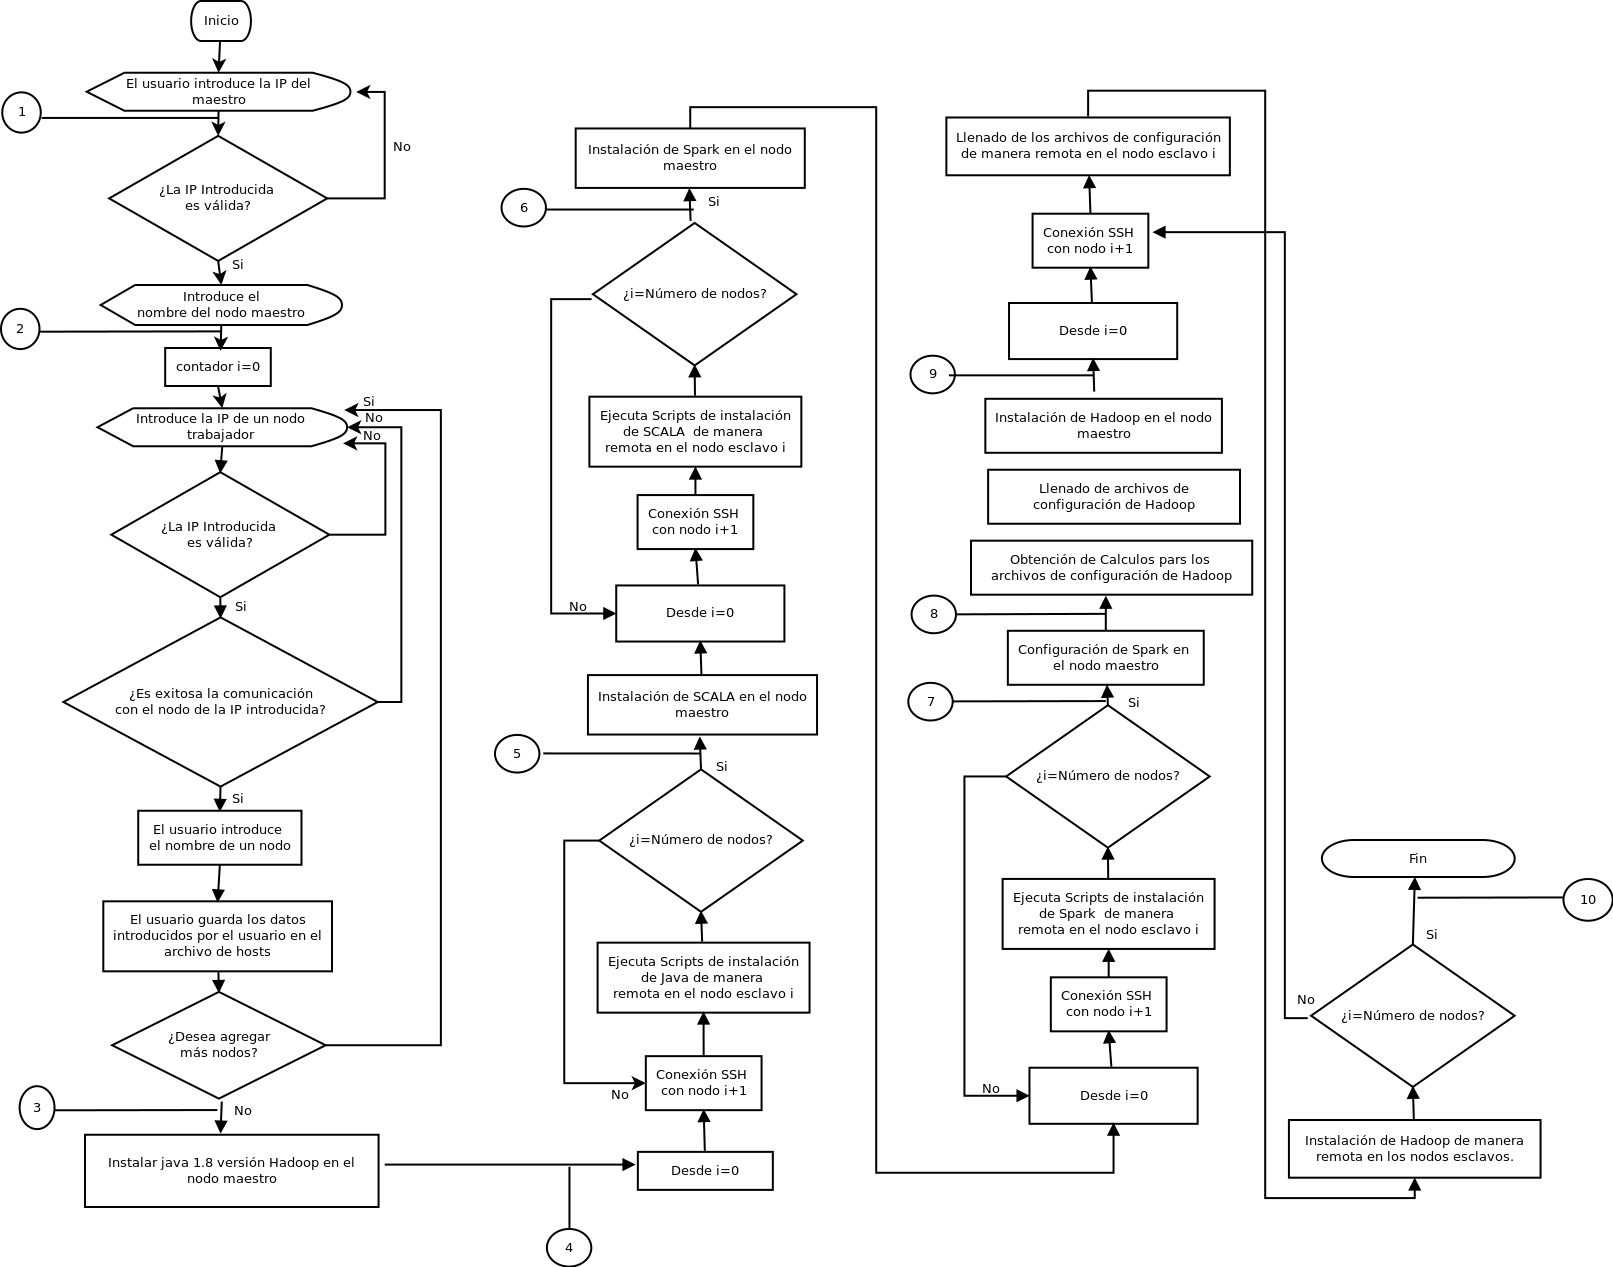
\includegraphics[width=1\textwidth]{capitulo5/images/diagramaflujoinstalador.png}
		\caption{Diagrama de flujo del instalador.}
		\label{fig:diagramaFlujo}
	\end{center}
\end{figure}
\newpage
El listado de pasos del instalador tal como se puede observar en el diagrama de flujo, si se compará contra el indice del Manual de Instalación de \emph{Luminus}, se podría confirmar que estos en general siguen el mismo proceso y secuencia.
\\
Si además se evaluá su flujo paso a paso, sería posible ver que el \emph{Instalador} sigue el mismo flujo que el \emph{Manual de Instalación de Luminus} en cada uno de los pasos, exceptuando que, para algunos de ellos es necesario realizar algunas adecuaciones y consideraciones para que puedan ser ejecutadas desde código y no directamente por el usuario.
\\
Una vez establecido que el listado de pasos es el mismo,  faltaría conocer cuales son las consideraciones adicionales que se tienen que tomar en cuenta el instalador para poder operar en relación a hacerlo de manera manual las cuales se encuentran listadas en la sección \ref{explicacion}.
\\
En Resumen, ambos medios hacen lo mismo, ejecutando los mismos pasos solo que uno de ellos lo  realiza de manera automática y el otro requiere intervención del usuario en cada uno de sus pasos. La principal diferencia entre ambos es que el usuario en este instalador no puede manejar las excepciones de manera directa y se busca que el instalador pueda arrojar el menor numero de errores posible y considerar la mayor cantidad de casos,de manera que a medida de nuestras posibilidades, estos puedan ser manejados y resueltos desde el propio código del instalador.
\\
El \emph{Manual de instalación de Luminus} tiene documentados cada uno de los pasos necesarios para el funcionamiento describiendo:
\begin{itemize}
	\item Que hace cada uno de los pasos en la instalación
	\item Como lo hace
	\item Como se configura
	\item Que significa cada uno de los parámetros de entrada
	\item Entre otros
\end{itemize}
Es posible que en caso de existir, dudas, interés o algún problema con el \emph{Instalador de Luminus} se recurra a el \emph{Manual de instalación de Luminus} a consultar la documentación de los pasos que hace.
\\
Por otro lado, también es de utilidad en caso de desear conocer el detalle de cuales son los pasos para instalar alguna de las paqueterias que son instaladas por el instalador, o bien, lo que se requiere para replicar su instalación en los nodos de datos/replica, toda esta información se encuentra en el  \emph{Manual de instalación de Luminus}. por lo que puede ser utilizado como referencia.
\\
Una de las consideraciones importantes que este instalador toma en cuenta es que todos los pasos puedan ser ejecutados desde el nodo maestro, para que con esto, sea mas sencillo para el usuario final, en lugar de realizar cada uno de los pasos en los diferentes equipos de computo involucrados esto lo hace haciendo uso de un programa llamado SSH el cual le permite realizar todas las conexiones pertinentes entre los diferentes equipos de computo involucrados.
\\
Esto con el objetivo de que el nodo maestro pueda comunicarse remotamente a los nodos de datos/replica y realizar las instalaciones y configuraciones pertinentes.
\\
Las entradas y salidas del diagrama de flujo con respecto a la intervención del usuario en el manual de instalación actual de Luminus, disminuyen demasiado lo cual será detallado y revisado a profundidad en la sección \ref{desarrollo}.
\\
\subsubsection{Explicación del funcionamiento del instalador}\label{explicacion}
A continuación se da una descripción a gran escala de como el instalador lleva a cabo su trabajo en cada uno de los pasos, considerando de manera general, un paso como los que vienen indicados en el diagrama,con un circulo el cual contiene el numero de paso.
\begin{enumerate}
	\item \label{paso1}Este paso consiste en comenzar el instalador y llevar a cabo la primera tarea para que inicie su ejecución la cual seria, solicitar la dirección IP de la computadora que tendrá el papel de nodo maestro. 
	\\
	Como tal no es un paso de ejecución o completa ninguna tarea en particular, sin embargo, sirve para marcar el inicio de la ejecución del instalador, e identificar en caso de fallo que ya se había intentado realizar la instalación anteriormente.
	\item \label{paso2} Este paso, permite introducir los datos que identifican al nodo maestro, por lo que, una vez completado este paso se tiene conocimiento de la IP del nodo maestro así como del nombre que se le quiere dar como identificador a este nodo.
	\\
	La información de la IP introducida pasa a través de una expresión regular, la cual, permite validar que efectivamente tiene las características de una dirección IP, por ejemplo: 4 octetos, caracteres numéricos, octetos separados por punto, valor de un octeto no mayor a 255, etc. en caso de que los datos recibidos no sean aprobados en esta validación se solicita al usuario que la ingrese nuevamente.
	\\
	Si la IP introducida es correcta, se valida que al realizar un ping exista una respuesta, esto para verificar que efectivamente se trate de una IP accesible y asignada a algún equipo de computo dentro de la red.
	\\
	Una vez hechas ambas validaciones se solicita un nombre de nodo maestro, para identificar al nodo que se acaba de agregar, a continuación se permite al usuario continuar con el instalador y lo posiciona en el punto 2.
	
	\item El siguiente paso, consiste en realizar una operación muy parecida a la que se lleva a cabo en el punto 2, pero en lugar de ser para el nodo maestro se ejecuta para los nodos de datos/replica por lo que, al poder existir más de un nodo de datos/replica esta sección es capaz de repetirse hasta que el usuario haya terminado de ingresar todos los nodos de datos/replica que desee.
	\\
	La información de la IP introducida para cada uno de los nodos de datos/replica pasa a través de una expresión regular, la cual, permite validar que efectivamente tiene las características de una dirección IP, por ejemplo: 4 octetos, caracteres numéricos, octetos separados por punto, valor de un octeto no mayor a 255, etc. en caso de que los datos recibidos no sean aprobados en esta validación se solicita al usuario que la ingrese nuevamente.
	\\
	Si la IP introducida es correcta, se valida que al realizar un Ping exista una respuesta, esto para verificar que efectivamente se trate de una IP accesible y asignada a algún equipo de computo dentro de la red.
	\\
	Una vez hechas ambas validaciones se permite al usuario indicar el identificador que desea dar a este nodo de datos/replica, y posterior a ello tiene la opción de seleccionar si quiere ingresar un nuevo nodo de datos/replica. En caso de indicar que desea hacerlo entonces esta sección se repetirá para el nuevo nodo, cuando el usuario ya no quiera agregar mas nodos de datos/replica se le permitirá continuar con el instalador y lo posiciona en el punto 3. 
	\item Cuando ya se tienen todas las configuraciones necesarias para iniciar la instalación de los paquetes necesarios, el primero en instalarse es JAVA instalándolo de primera instancia en el nodo maestro. 
	\\
	Debido a que muchos usuarios tienen otra instalación de JAVA en sus equipos de computo requerida para otras aplicaciones instalar la versión que se necesita para el instalador, tiene que hacerse de forma independiente, creando una nueva carpeta para su instalación.
	\\
	Por lo que la versión de JAVA requerida, no sería la principal del equipo y tampoco empataría con otras versiones disponibles esto quiere decir que no se intentaría actualizar las versiones que se tengan en la maquina. 
	\\
	Consultando otras herramientas que también ofrecen soluciones de Big Data como \emph{Cloudera}, la solución mencionada anteriormente es la solución que se implementa para esta problemática. por lo que, tomando como referencia el análisis hecho y el conocimiento de que se trata de una posibilidad ya probada por otros sistemas se recurrió a hacerlo de esta misma forma.
	\\ 
	Cuando la versión de JAVA se encuentre correctamente instalada en el nodo maestro, se coloca la instalación en el punto 4.
	\item Posteriormente se procede a instalar de manera distribuida para cada uno de los nodos que se tienen la paquetería de JAVA, utilizando la misma estrategia propuesta para el nodo maestro, haciendo uso de una carpeta adicional para poder diferenciar esta instalación de otras que pudiera tener el equipo de computo. \\
	Esta instalación se lleva a cabo comunicándose con el nodo de replica/datos haciendo uso de SSH y con esto, hace el envió de lo requerido para ejecutar la instalación y posteriormente se envían las instrucciones en forma de pasos para la terminal para que esta los ejecute y al finalizar JAVA quede instalado, desde cada uno de los nodos de datos/replica indicados en el paso 2 cuando son invocados para instalación.\\
	Una vez que esta instalación se concluye de forma satisfactoria se coloca el instalador en el punto 5.
	\item Otra tecnología importante a considerar durante la instalación es SCALA el cual es un lenguaje de programación moderno multi-paradigma sobre el que pueden ser implementadas muchas operaciones de minería de datos y algoritmos de análisis de datos de gran volumen.\\
	Esta instalación primero se efectuá en el nodo maestro y posteriormente es replicada haciendo uso de SSH a cada uno de los nodos de datos/replica. \\
	En lo que respecta a esta instalación en particular solo fue necesario pasar cada uno de los pasos descritos en el manual de instalación a el instalador sin tener que hacer cambios en la lógica de funcionamiento, ni considerar excepciones. \\
	Una vez que esta instalación se concluye de forma satisfactoria se coloca el instalador en el punto 6.
	\item Lo siguiente que hace el instalador en este punto es: Instalar Apache Spark tanto en el nodo maestro como en los nodos de datos/replica.\\
	Para llevar a cabo esta instalación Apache Spark requiere que un par de archivos de configuración sean modificados, por lo que el instalador crea archivos "Plantilla" Los cuales se crean escribiendo los datos correspondientes a la instalación que se esta efectuando. Es importante que se haga de esta forma, ya que, cada instalación llena estos archivos con información diferente.\\
	La información que sea escrita en los archivos antes mencionados depende directamente de la información que fue introducida en los pasos \ref{paso1} y \ref{paso2} como identificadores de los nodos ya que, Apache Spark debe ser capaz de identificarlos y para ello se utilizan los identificadores proporcionados.\\
	\\
	Una vez que estos archivos son generados de forma satisfactoria se coloca el instalador en el punto 7.
	\item 
	Los archivos "Plantilla" que se generan así como el archivo de instalación de Apache Spark es replicado hacia los nodos de datos/replica, para que estos puedan concretar sus propias instalaciones, y los archivos "Plantilla" generados reemplazan a el archivo original que se encuentra en el directorio sin ningún tipo de configuración estos cambios se realizan tanto para el nodo maestro como para los nodos de datos/replica. 
	\\
	Por otro lado, también es necesario modificar los archivos de variable de entorno, para que el nodo maestro sea capaz de reconocer a Apache Spark como una variable de entorno y con esto tener acceso a el desde cualquier punto del sistema operativo entre otras ventajas que son ofrecidas por esta configuración.
	\\
	una vez hecho esto, se tiene todo lo necesario para poder iniciar Apache Spark unicamente haciendo uso del comando \emph{start-all.sh}.
	\\
	Cuando estas configuraciones hayan sido efectuadas de manera exitosa, se coloca el instalador en el punto 8.
	\item La última tecnología considerada por el instalador es Apache Hadoop, esta es una tecnología que con el proceso de instalación resulta la mas pesada de todas las anteriormente contempladas. \\
	Como primer punto es importante instalarlo de manera satisfactoria en el nodo maestro, para ello , al igual que en Apache Spark se requiere el manejo de archivos "Plantilla", ya que se hacen bastantes configuraciones en diferentes archivos. \\
	Las configuraciones requeridas, dependen de la información propia del equipo de computo que alojará la instalación, por lo que es necesario, correr un script que obtiene información del sistema operativo la procesa y obtiene la que es importante para los archivos de configuración.
	\\
	además se requieren otro tipo de configuraciones, por ejemplo datos proporcionados en los pasos \ref{paso1} y \ref{paso 2} y otro conjunto de configuraciones de como se espera que sea el funcionamiento Hadoop por ejemplo, delimitadores dentro de un conjunto permitido de valores para que el ambiente pueda ser adaptado a diferentes necesidades.
	\\
	Cuando se tienen todos los datos necesarios para la configuración de los archivos, Se construyen los archivos de configuración "Plantilla" con los datos recabados en las secciones correspondientes.
	\\
	Una vez que se tienen los archivos plantilla antes mencionados, se reemplaza en el nodo maestro los archivos de configuración por los archivos "Plantilla".
	\\
	también se agrega la información de Apache Hadoop a las variables de entorno para este pueda ser accedido desde cualquier punto dentro del sistema operativo.\\
	Cuando estas configuraciones en el nodo maestro hayan sido efectuadas de manera exitosa, se coloca el instalador en el punto 9.
	\item Lo siguiente que hace el instalador en este punto es: Instalar Apache Hadoop en los nodos de datos/replica.\\
	Para ello es necesario replicar los archivos de configuración "Plantilla" generados a cada uno de los nodos de datos/replica dentro de la red distribuida.\\
	Realizar la instalación de Apache Hadoop en cada uno de los nodos de datos/replica y reemplazar los archivos de configuración por defecto con los archivos de "Plantilla" que se tienen para realizar estas configuraciones.
	\\
	Una vez que esta instalación se concluye de forma satisfactoria en los nodos de datos/replica, se coloca el instalador en el punto 10.\\
	es necesario ponerlo en este punto, ya que, si alguien desea volver a iniciar el instalador, con esta información el instalador será capaz de saber que ya había terminado de ejecutar todas las tareas y no quedaban tareas restantes, por lo que se regresará la solicitud notificando que esta instalación ya había terminado con éxito anteriormente.\\
	Este es el ultimo paso del instalador y una vez que este termina entonces termina la ejecución del instalador.\\ 
\end{enumerate}
Cada uno de los pasos, descritos anteriormente, al ser completado, marca un estatus de progreso en la ejecución del instalador, este permite que , si el instalador o el proceso de instalación presenta alguna falla o problemática que no le permita continuar con su ejecución, será posible volver a iniciar el instalador y que este reconozca el ultimo punto donde estuvo trabajando para continuar a partir de ese punto y re intentar la instalación. Pero sin comenzar desde el principio y conservando los pasos que resultaron exitosos.
\\
  
\section{Desarrollo}\label{desarrollo}
El codigo fuente que se escribió en Shell Script contiene los siguientes pasos que se enuncian en el manual de instalación de \emph{Luminus}.
\begin{verbatim}
1 Instalación de Apache Spark en el nodo maestro
    1.1. Instalación de la paquetería de java 
    1.3. Instalación de Spark
    1.3.1. Configuración maestro
2. Instalación de Apache Spark en los nodos de datos
    2.1. Instalación de la paquetería de java en los nodos de datos
    2.3. Instalación de Spark en los nodos de datos
         2.3.1. Configuración 
3. Puesta en funcionamiento
    3.1. Configuraciones para poner en funcionamiento Apache Spark en la red distribuida
    3.2. Puesta en funcionamiento del cluster manejado por el Servidor Apache Spark
4. Instalación de Apache Hadoop en el nodo maestro
    4.1. Instalación de Hadoop 
        4.1.1. Configuración
        4.1.2. Archivos de configuración
5. Instalación de Apache Hadoop en los nodos de datos
    5.1. Instalación de Hadoop en los nodos de datos
        5.1.1. Configuración
\end{verbatim}
Algunos pasos enunciados en el manual de instalación de \emph{Luminus}, no se encuentran detallados en esta parte, por lo que a continuación se procederá a explicar cuales son estos puntos y la razón por la cual no forman parte del instalador.
Estos pasos, tendrían que ser resueltos de manera manual por el usuario final durante el proceso de instalación.
\begin{verbatim}
1 Instalación de Apache Spark en el nodo maestro
    1.2. Instalación de la paquetería de SSH
         1.2.1. Configuración
         1.2.2. Conexión
2. Instalación de Apache Spark en los nodos de datos         
    2.2  Instalación de la paqueteria SSH en los nodos de datos
6. Puesta en funcionamiento
		6.1. Puesta en funcionamiento del Cluster manejado por el Servidor Apache Hadoop
		6.2. Subir un archivo al HDFS
\end{verbatim}

\subsubsection{Instalación de la paquetería de SSH}
Para el instalador, es muy importante que tanto el nodo maestro como los nodos de datos/replica tengan instalado y configurado correctamente SSH ya que en caso de no ser así, no se podría establecer la conexión entre los nodos y por lo tanto sería imposible realizar la instalación de manera distribuida a cada uno de los nodos.
\\
Por lo que se requiere que se encuentre correctamente instalado, el servicio se encuentre iniciado al momento y que además se permitan conexiones de tipo root en cada uno de los nodos.
\\
Por otro lado, se requiere la creación de una llave keygen en el servidor SSH para que las contraseñas que se utilicen para establecer las conexiones sean seguras y se encuentren cifradas esto con el fin de proteger los datos internos de la empresa y la información que viaja a través de la red, permitiendo cambiar entre los algoritmos de cifrado a utilizar y la longitud con la que las llaves son generadas.
\\
como segundo punto, simplifica el numero de pasos del instalador, ya que de esta manera, no se necesita introducir las contraseñas de root para establecer las conexiones al momento de llevar a cabo el proceso de instalación. 
\\
\subsubsection{Puesta en funcionamiento}
Una vez que se terminan de hacer todas las configuraciones básicas consideradas en el proyecto y se tienen todos los programas necesarios para el mismo, el instalador termina, y con esto es suficiente para que la plataforma de Big Data, este en operación, sin embargo, puede presentarse el caso en que un usuario final requiera realizar mas configuraciones especificas.\\
En este caso, el usuario, deberá realizar estas configuraciones manualmente antes de poner en funcionamiento, la totalidad del sistema. por lo que, las configuraciones de esta sección tendrían que ser hechas por el usuario, para considerar estas excepciones.\\
Además de que solo se trata unicamente de 2 pasos los cuales además solo pueden ser hechos en una única ocasión luego de la instalación, y al tratarse de algo tan delicado, por eso lo dejamos como un paso independiente que se considera no es apropiado automatizar.
\\
\subsubsection{Consideraciones adicionales}
A continuación se muestra una tabla, con el listado del número de pasos que implica hacer la instalación mediante el \emph{Manual de instalación de Luminus} de estas tecnologías, con respecto al número de pasos que implica hacerlo mediante el instalador. 
\\
\begin{table}[H]
\begin{tabular}{|l|l|l|}
\hline
Tarea                                                   & \begin{tabular}[c]{@{}l@{}}Número de pasos en el \\ manual de instalación\end{tabular} & \begin{tabular}[c]{@{}l@{}}Número de pasos \\ en el instalador\end{tabular} \\ \hline
Instalación de la paquetería java en el Nodo Maestro    & 2 pasos                                                                                   & -----                                                                          \\ \hline
Instalación de la paquetería SSH en el Nodo Maestro     & 9 pasos                                                                                   & 9 pasos                                                                        \\ \hline
Instalación de Spark en el Nodo Maestro                 & 7 pasos                                                                                   & ----                                                                           \\ \hline
Instalación de la paquetería java en los nodos de datos & 2 pasos                                                                                   & ----                                                                           \\ \hline
Instalación de la paquetería SSH en los nodos de datos  & 4 pasos                                                                                   & 4 pasos                                                                        \\ \hline
Instalación de Spark en los nodos de datos              & 7 pasos                                                                                   & ----                                                                           \\ \hline
Instalación de Apache Hadoop en el nodo maestro         & 20 pasos                                                                                  & ----                                                                           \\ \hline
Instalación de Apache Hadoop en los nodos de datos      & 5 pasos                                                                                   & ----                                                                           \\ \hline
Puesta en funcionamiento (Pasos necesarios)             & 2 pasos                                                                                   & 2 pasos                                                                        \\ \hline
Pasos adicionales del instalador                        & ----                                                                                      & 5 pasos                                                                        \\ \hline
TOTAL                                                   & 58 pasos                                                                                  & 20 pasos                                                                       \\ \hline
\end{tabular}
\end{table}
Como se puede notar, el número de pasos necesarios disminuyo considerablemente y esto debido a que algunas de las secciones necesarias de llevar a cabo en el \emph{Manual de Instalación de Luminus} haciendo uso del instalador ya no son necesarias.
\\
Por otro lado, muchos de los pasos enlistados para la configuración de SSH, puede que algún usuario ya los tenga realizados de instalaciones o configuraciones previas, con lo que en este caso solo sería necesario llevar a cabo \textbf{7 pasos} para tener un ambiente de Big Data, funcionando en su totalidad.\\
Pero, incluso no existiendo este caso ideal, unicamente seria necesario ejecutar el \textbf{34\% de los pasos originales}. 
\\
El código fuente actual de este desarrollo se puede consultar en el anexo \ref{anexob}.
\\
Con esto, se logro que el usuario final realice menos pasos de los que tendrían que llevarse a cabo si se siguiera el \emph{Manual de Instalación de Luminus}directamente. 
\\
\subsubsection{Manejo de versionamiento de Software involucrado}
Debido a que las versiones de los software a utilizar pueden estar en constante cambio, y que en el momento de ocurrir una actualización de versión en alguno de los software requeridos por el instalador podrían ocurrir fallas en el instalador al no soportar los cambios realizados.
\\
Por lo que, se propone utilizar versiones estáticas de el software requerido por el instalador, para que de esta manera se pueda garantizar, actualizar las versiones del instalador en paralelo con las actualizaciones que se realicen sobre la paquetería necesaria para su operación.
\\
De esta forma, se puede garantizar, que el instalador sea capaz de soportar la versión que por el mismo descargue, y no por una actualización del repositorio origen este deje de funcionar de manera correcta o incluso, no existiría la necesidad de buscar entre diferentes servidores para localizar donde se encuentre disponible el archivo que se esta buscando, ya que la información que cada uno de estos servidores independientes tiene disponible no es gestionada por \emph{Luminus}.
\\
Al momento de descargar el instalador desde el servidor que lo aloje, se descargaran también los paquetes requeridos de las tecnologías a utilizar de esta versión.
\\
Dichos paquetes se irían actualizando en el servidor de versiones de \emph{Luminus} para que, con ello, para cada nueva versión que se genere de \emph{Luminus} se actualice también la paquetería necesaria.
\\
\\
Por ejemplo, para la primera versión de este instalador se utilizarían las siguientes versiones de los paquetes a instalar:
\begin{itemize}
	\item Java Open JDK 1.8
	\item Scala 2.6.11
	\item Spark 2.7
	\item Hadoop 3.1.1
	
\end{itemize}
\section{Pruebas}
Se presenta a continuación una prueba demostrativa del funcionamiento del instalador y como este es operado por el usuario final: Que es lo que el ve, en que momento se despliegan los pasos, cuales son las tareas que tiene que llevar a cabo, etc.
\\
Para la documentación de esta prueba se procede a listar paso por paso lo que el instalador va haciendo, además se agrega evidencia de como esto se visualiza en las salidas arrojadas por el instalador.
\\
El instalador cuenta con 10 pasos importantes durante su ejecución de acuerdo con el diagrama de flujo que se muestra en la imagen \ref{fig:diagramaFlujo} y con la descripción de los pasos del instalador que se realiza en la sección \nameref{explicacion} se tomarán como referencia estos pasos para clasificar cada uno de los elementos del instalador, por lo que en esta sección no se hará mucha referencia a la manera en que estos operan ya que esta información puede ser encontrada en la sección \ref{explicacion}, sino mas bien en como el usuario participa en cada una de estas secciones y como es que estas secciones se visualizan para el usuario final.
\\
\subsubsection{Paso 1 y Paso 2}
Para comenzar, el instalador será ejecutado solamente desde la máquina que ocupe el rol de nodo maestro de la red distribuida haciendo uso de su terminal con privilegios de super usuario y ejecutando el siguiente comando. 
\\
\begin{verbatim}
./lum-ins.sh
\end{verbatim}
\begin{figure}[H]
	\hypertarget{fig:ejecucion}{\hspace{1pt}}
	\begin{center}	
		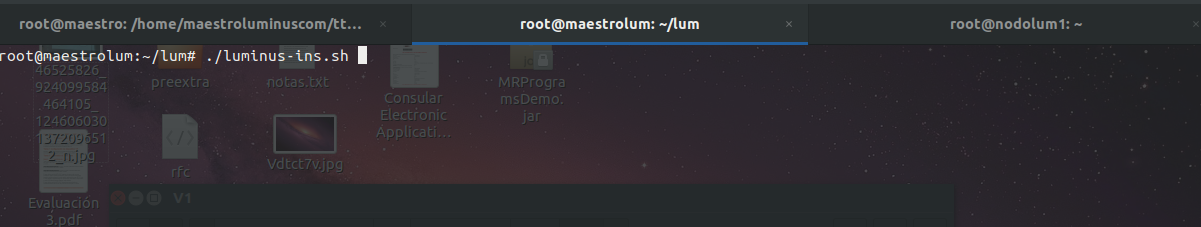
\includegraphics[width=.7\textwidth]{capitulo5/images/ejecucion.png}
		\caption{Ejecución del instalador.}
		\label{fig:Ejecucion del instalador}
	\end{center}
\end{figure}
Éste preguntará al usuario por la IP del nodo maestro, Luego preguntará por las IPs de los nodos que conformarán la red distribuida. \\
Cuando una dirección IP es introducida, el instalador valida que efectivamente se trate de un formato de dirección IP valida, revisando sus características como cadena haciendo uso de una expresión regular, en caso de no tratarse de una dirección IP valida, entonces, se indicara el error como se muestra en la figura \ref{fig:hostnoencontrado} para que el usuario pueda intentar nuevamente introducirla y no se almacena ningún tipo de información referente a este host erroneo.
\\
Además, el instalador hará un ping para comprobar si hay conexión con el nodo cuya IP se desea agregar a la red distribuida. Si hay respuesta por parte del nodo en cuestión, se pregunta el nombre con el que se desea almacenar este nodo y se procede a almacenar estos datos en un archivo.
\\
\begin{figure}[H]
	\begin{center}	
		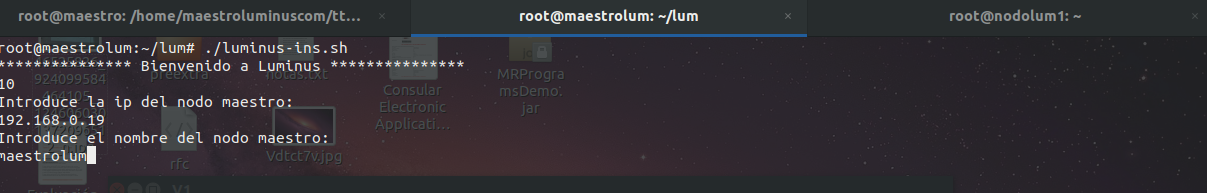
\includegraphics[width=.7\textwidth]{capitulo5/images/ipmaestro.png}
		\caption{IP del Maestro.}
		\label{fig:maestro}
	\end{center}
\end{figure}
\begin{figure}[H]
	\begin{center}	
		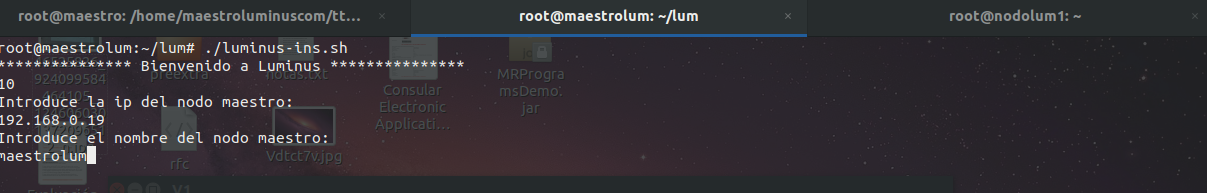
\includegraphics[width=.7\textwidth]{capitulo5/images/ipmaestro.png}
		\caption{IP del nodo datos/replica.}
		\label{fig:esclavo}
	\end{center}
\end{figure}
finalmente, una vez que el nodo es agregado, se le pregunta al usuario si desea agregar otro nodo como se muestra en la figura \ref{fig:nuevonodo}. Si su respuesta es afirmativa, este proceso se repite. 
\begin{figure}[H]
	\begin{center}	
		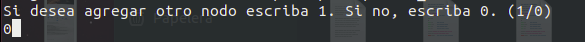
\includegraphics[width=.7\textwidth]{capitulo5/images/copiadohosts.png}
		\caption{Nuevo nodo}
		\label{fig:nuevonodo}
	\end{center}
\end{figure}
El instalador, es capaz de detectar cuando la IP introducida no corresponde a un Host que se encuentre dentro de la red local y notifica al usuario experto de esto, como se muestra en la figura \ref{fig:hostnoencontrado} además de no realizar ningún tipo de almacenamiento de información referente a este host, erroneo.
En esta situación, el usuario puede volver a introducir los datos del host una vez que este los verifique, o bien, introducir los datos de algún otro host luego de comprobar que el host introducido no es accesible desde el nodo maestro y que los datos introducidos por el fueron correctos.
\\
\begin{figure}[H]
	\hypertarget{fig:hostnoencontrado}{\hspace{1pt}}
	\begin{center}	
		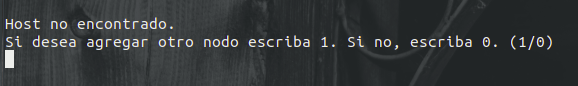
\includegraphics[width=.7\textwidth]{capitulo5/images/hostno.png}
		\caption{El usuario introdujo la IP de un host no encontrado.}
		\label{fig:hostnoencontrado}
	\end{center}
\end{figure}
\subsubsection{Paso 3}
Posteriormente, cuando ya no se deseen agregar más nodos, el instalador comenzará su trabajo llevando a cabo la instalación de los paquetes necesarios, en cada uno de los nodos que conforman la red distribuida.\\
En este punto el usuario experto, deja de tener mucha injerencia en el proceso de instalación y solo tiene que esperar que los pasos vayan siendo completados de manera exitosa. \\
Por lo que ya no se verá tanta participación por parte del usuario experto a partir de este paso en el instalador y los posteriores.\\
Lo primero que se instala es la Paquetería de java comenzando por hacerlo desde el nodo maestro. Como se muestra en la imagen \ref{fig:javamaestro} es necesario ejecutar la descompresión del archivo correspondiente a este paquete que viene con el instalador, en el nodo maestro para posteriormente, proceder a realizar la instalación del mismo.\\
como se menciona en la sección \nameref{explicacion} se busca que, incluso en caso de que alguno de los equipos de computo involucrados en la red distribuida tengan instalada alguna versión de Java, no se tenga ningún tipo de conflicto con ella, y en su lugar, puedan vivir ambas instalaciones en el equipo de computo.
\begin{figure}[H]
	\hypertarget{fig:javamaestro}{\hspace{1pt}}
	\begin{center}	
		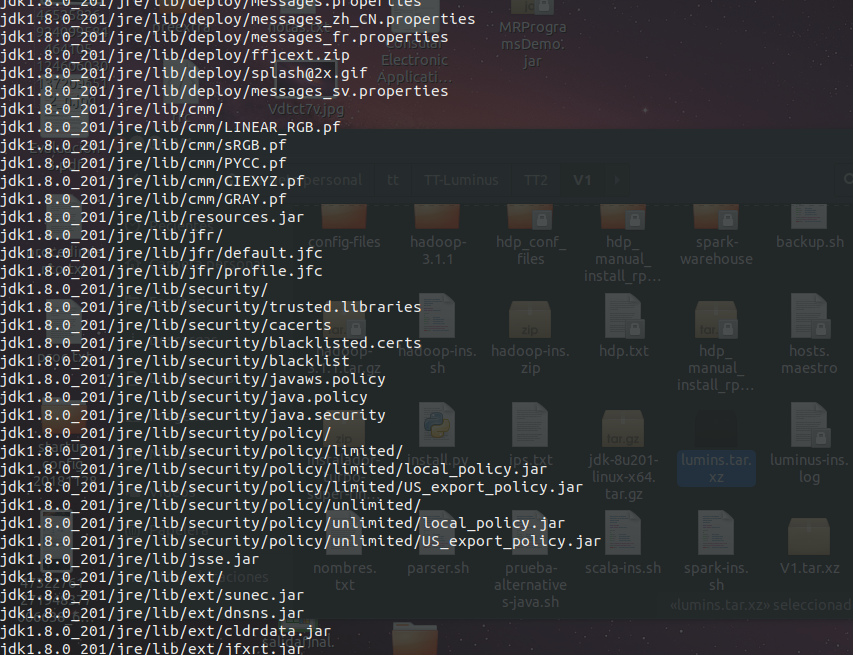
\includegraphics[width=.7\textwidth]{capitulo5/images/instalacionjavamaestro.png}
		\caption{Instalación de Java en el Nodo Maestro.}
		\label{fig:javamaestro}
	\end{center}
\end{figure}
\subsubsection{Paso 4}
Una vez que la paquetería de JAVA esta correctamente instalada en el nodo maestro, se procede a instalarla en cada uno de los nodos de datos/replica que fueron configurados.\\
Es necesario hacer un copiado mediante el uso de SSH de los archivos como se puede apreciar en la figura \ref{fig:copiajava}. y cuando estos archivos ya se encuentran en cada uno de los nodos de datos/replica, entonces se procede a hacer la descompresión de estos de la misma forma en que lo efectuá en el nodo maestro, y puede ser observado en la imagen \ref{fig:javamaestro}.
\\
Cuando los archivos se encuentran descomprimidos, se hace la instalación de java en cada uno de los nodos, esto se hace de la misma forma que en el nodo maestro. la cual es: crear una carpeta que contenga la versión de JAVA que se pretende instalar, para que esta versión pueda vivir en el equipo de computo,ademas de que si se encuentra alguna otra versión de JAVA instalada en el equipo de computo no se genere ningún conflicto con ella y ambas puedan funcionar estar en funcionamiento dentro del equipo de computo.
\begin{figure}[H]
	\hypertarget{fig:copiajava}{\hspace{1pt}}
	\begin{center}	
		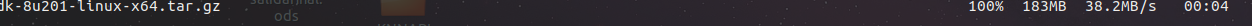
\includegraphics[width=1\textwidth]{capitulo5/images/copiaeinstalacionjava.png}
		\caption{Copiado de los archivos correspondientes de java.}
		\label{fig:copiajava}
	\end{center}
\end{figure}
\subsubsection{Paso 5}
Posterior a la instalación de Java se procede a realizar la instalación de Scala, la cual se lleva a cabo de una forma muy similar a como se hizo la instalación de Java.
\\ 
Es necesario descargar el archivo comprimido de Scala desde la liga que lo contiene, para esta versión del instalador en el nodo maestro como se muestra en la figura \ref{fig:descarga}. 
\begin{figure}[H]
	\hypertarget{fig:descarga}{\hspace{1pt}}
	\begin{center}	
		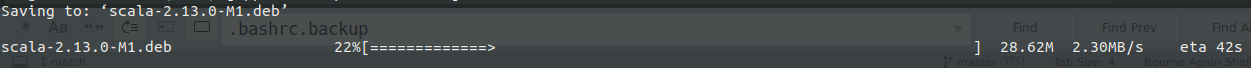
\includegraphics[width=.7\textwidth]{capitulo5/images/descargascala.png}
		\caption{Descarga de Scala en el nodo Maestro}
		\label{fig:descarga}
	\end{center}
\end{figure}
Posteriormente se procede a descomprimir los archivos de Scala descargados al nodo maestro y realizando la instalación de los mismos como se muestra en la figura \ref{fig:scala} .
Para esta instalación no es necesario realizar configuraciones adicionales o algún tipo de adecuación y se siguen los mismos pasos de el \emph{Manual de instalación de Luminus}
\begin{figure}[H]
	\hypertarget{fig:scala}{\hspace{1pt}}
	\begin{center}	
		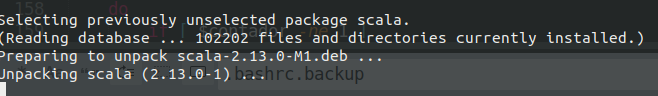
\includegraphics[width=.7\textwidth]{capitulo5/images/instalacionscalam.png}
		\caption{Instalación de Scala}
		\label{fig:scala}
	\end{center}
\end{figure}
\subsubsection{Paso 6}
Cuando la instalación esta completa en el nodo maestro, se envía el archivo .deb a cada uno de los nodos de datos/replica haciendo uso de SSH como se muestra en la figura \ref{fig:scalaesclavo}.\\
Una vez que se encuentran en el nodo de datos/replica se procede a hacer la descompresión de este archivo y posteriomente a realizar la instalación como se muestra en la figura \ref{fig:scala} 
\begin{figure}[H]
	\hypertarget{fig:scalaesclavo}{\hspace{1pt}}
	\begin{center}	
		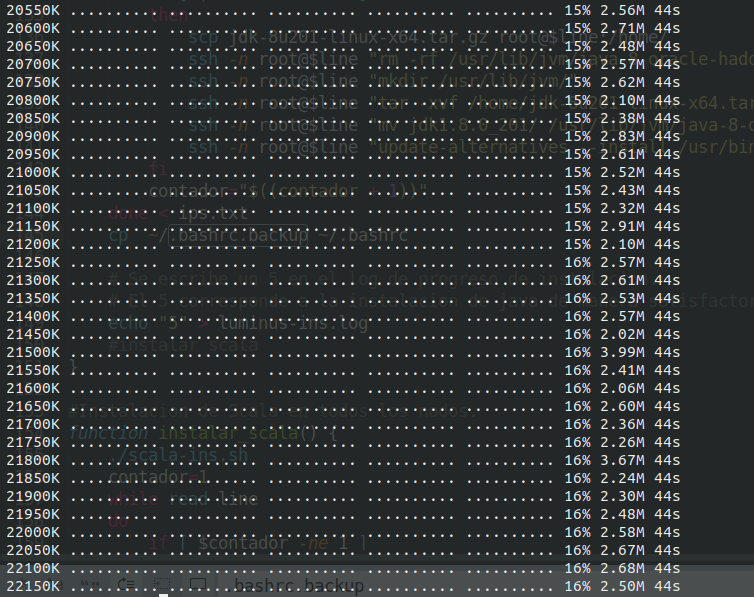
\includegraphics[width=.7\textwidth]{capitulo5/images/descargascalaesclavo.png}
		\caption{Descarga de Scala en los nodos de datos/replica.}
		\label{fig:scalaesclavo}
	\end{center}
\end{figure}
\subsubsection{Paso 7}
La siguiente tecnologia a instalar es Apache Spark, en este caso, de la misma manera que se realizo con las tecnologias anteriores se realiza la descarga de los paquetes necesarios en el nodo maestro tal como se muestra en la figura \ref{fig:sparkmaestro}
\begin{figure}[H]
	\hypertarget{fig:sparkmaestro}{\hspace{1pt}}
	\begin{center}	
		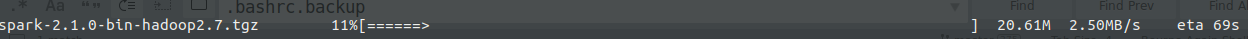
\includegraphics[width=.7\textwidth]{capitulo5/images/descargasparkmaster.png}
		\caption{Descarga de Apache Spark en el nodo maestro.}
		\label{fig:sparkmaestro}
	\end{center}
\end{figure}
Una vez que se tienen los paquetes necesarios, estos se descomprimen en el nodo maestro como se muestra en la figura \ref{fig:una1}. 
\begin{figure}[H]
	\hypertarget{fig:una1}{\hspace{1pt}}
	\begin{center}	
		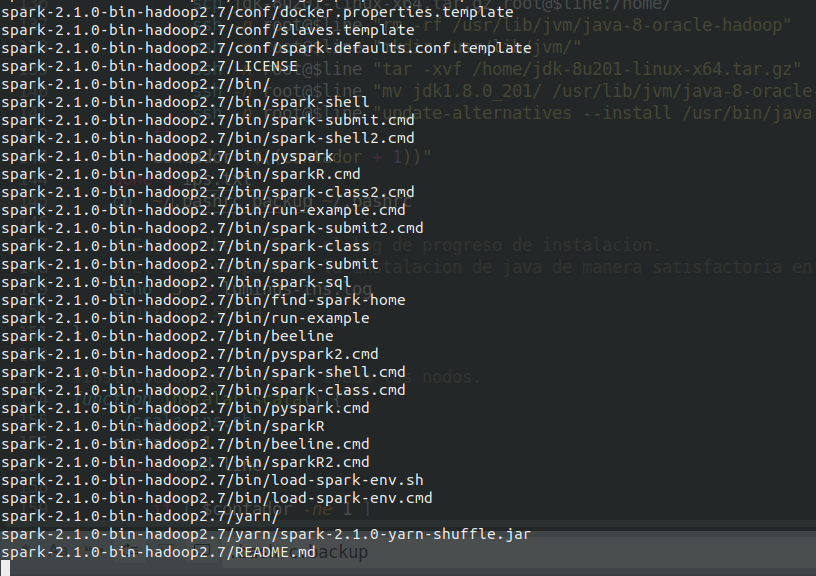
\includegraphics[width=.7\textwidth]{capitulo5/images/instalacionsparkmaestro.png}
		\caption{Instalación de Spark en el nodo Maestro.}
		\label{fig:una1}
	\end{center}
\end{figure}
\subsubsection{Paso 8}
Cuando la descompresión esta completada en el nodo maestro se procede a elaborar los archivos de configuración "Plantilla" para reemplazar a los archivos de configuración iniciales.
Una vez que Apache Spark queda correctamente instalado y configurado en el nodo maestro se procede a realizar lo mismo para los nodos de datos/replica. en este punto, se envía a los nodos esclavos tanto el .deb con los datos del comprimido de Apache Spark como los archivos de configuración generados, este paso se muestra en la figura \ref{fig:dos}
\begin{figure}[H]
	\hypertarget{fig:dos}{\hspace{1pt}}
	\begin{center}	
		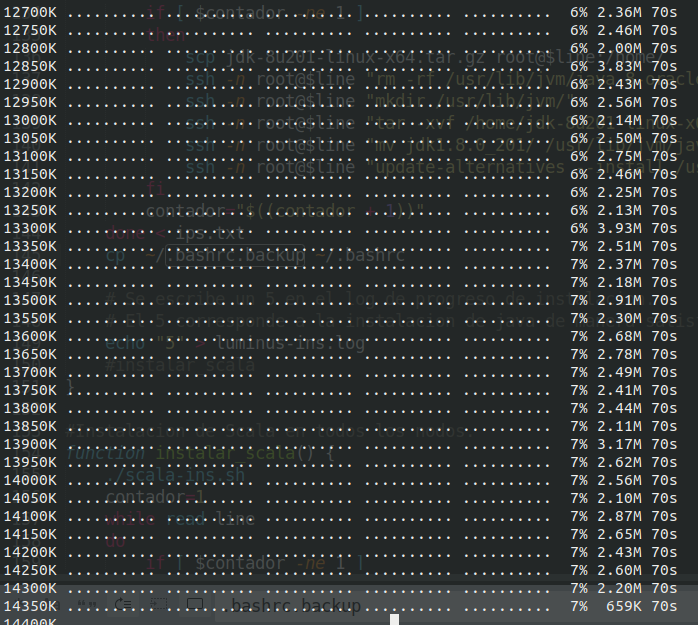
\includegraphics[width=.7\textwidth]{capitulo5/images/descargasparkesclavo.png}
		\caption{Descargar Spark en los nodos esclavos.}
		\label{fig:dos}
	\end{center}
\end{figure}
Al finalizar esta transferencia se procede a descomprimir los archivos de configuración enviados, reemplazar los archivos plantilla con los archivos de configuración y a realizar la instalación pertinente para cada uno de los nodos de datos.
\\
cuando este proceso termina, es suficiente con que se ejecute un paso manual adicional posterior a que este paso resulte exitoso en el instalador esto con el objetivo de iniciar las dependencias desde la consulta con privilegios de súper usuario el nodo maestro.\\
El paso es el siguiente:
\begin{verbatim}
./start-all.sh
\end{verbatim}
Lo cual iniciará todas las dependencias de Apache Spark como se muestra en la imagen \ref{fig:iniciaspark}
\begin{figure}[H]
	\hypertarget{fig:iniciaspark}{\hspace{1pt}}
	\begin{center}	
		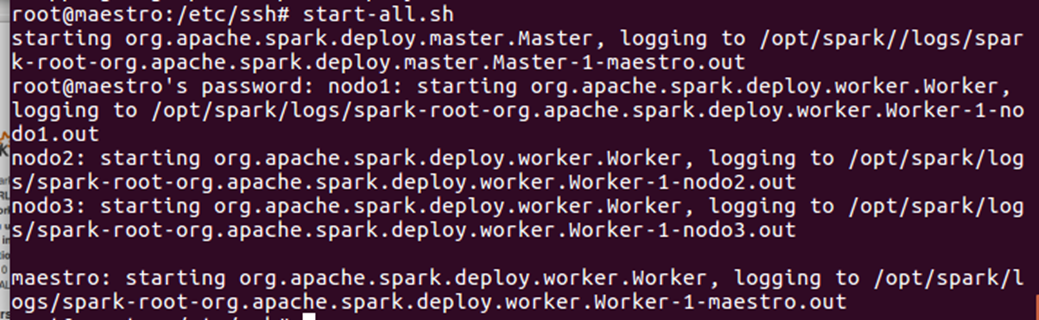
\includegraphics[width=.7\textwidth]{capitulo5/images/im27.png}
		\caption{Inicio de Apache Spark}
		\label{fig:iniciaspark}
	\end{center}
\end{figure}
Cuando se inicia Apache Spark en todos los nodos configurados mediante el paso mencionado ya se puede acceder a su vista de configuración de esta herramienta desde la que se puede controlar su funcionalidad.
\\
Esto, se puede hacer accediendo a la dirección ip del nodo maestro en el puerto 8080 con el siguiente comando desde un navegador web :
\begin{verbatim}
[Direccion IP Maestro]:8080
\end{verbatim}
si se desea acceder a esta vista desde el propio nodo maestro se puede reemplazar la dirección ip con la instrucción de hacerlo en local host como se muestra a continuación:
\begin{verbatim}
localhost:8080
\end{verbatim}
La salida entonces para esta dirección web será como se muestra en la imagen \ref{fig:salida} donde podremos ver toda la configuración de todos los nodos en la red distribuida para Apache Spark. 
\begin{figure}[H]
	\hypertarget{fig:salida}{\hspace{1pt}}
	\begin{center}	
		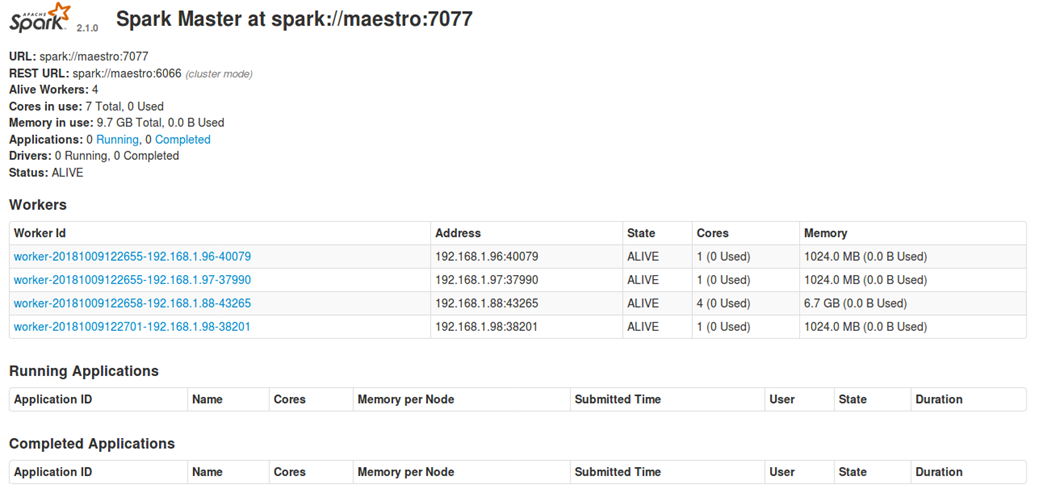
\includegraphics[width=.7\textwidth]{capitulo5/images/im28.png}
		\caption{Pantalla de configuración de Apache Spark}
		\label{fig:salida}
	\end{center}
\end{figure}
\subsubsection{Paso 9}
Otra tecnología que se instala es Apache Hadoop, para ello es necesario nuevamente, descargar los paquetes necesarios para efectuar esta instalación y posteriormente descomprimirlos dentro del nodo maestro, el proceso de descompresión puede ser observado en la figura \ref{fig:hadoopmaestro}.
\\
\begin{figure}[H]
	\hypertarget{fig:hadoopmaestro}{\hspace{1pt}}
	\begin{center}	
		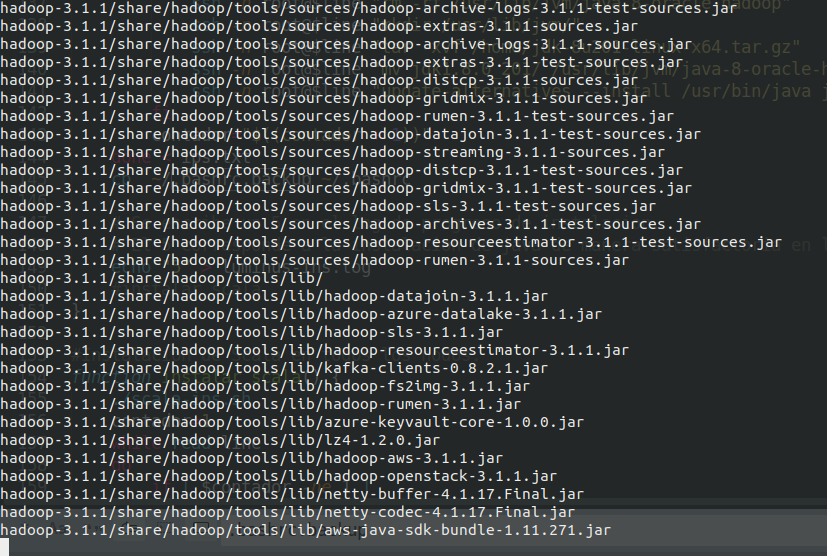
\includegraphics[width=.7\textwidth]{capitulo5/images/instalacionhadoopmaestro.png}
		\caption{Instalación de Hadoop en el nodo maestro}
		\label{fig:hadoopmaestro}
	\end{center}
\end{figure}
una vez que se termina la descompresión se procede a escribir los archivos de configuración "Plantilla" necesarios para estas tecnologías, estos se obtienen de: los datos proporcionados en los pasos 1 y 2 de este manual de instalación, algunos datos por defecto que se establecieron al definir el instalador y que tienen que ser replicados a los archivos de configuración cada vez que se haga una instalación de este tipo y algunos datos particulares de las maquinas donde se pretende establecer el ambiente de Big Data, para ello, se corre otro Script que permite obtener esta información para poder escribirla sobre a los archivos de configuración "Plantilla".
\\
una vez que los archivos de configuración "Plantilla" generados, estan listos, se procede a realizar el copiado de los mismos con las configuraciones establecidas reemplazando los archivos de configuración por defecto, este proceso de copiado se muestra en la figura \ref{fig:copiado}.
\begin{figure}[H]
	\hypertarget{fig:copiado}{\hspace{1pt}}
	\begin{center}	
		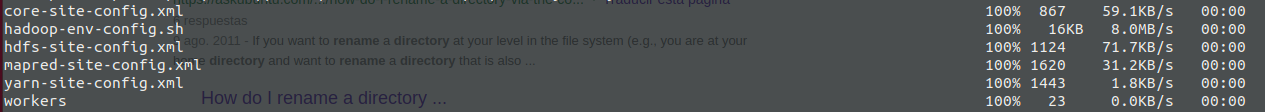
\includegraphics[width=.7\textwidth]{capitulo5/images/configuracionhadoopesclavo.png}
		\caption{Instalación de Hadoop en el nodo maestro}
		\label{fig:copiado}
	\end{center}
\end{figure}
\subsubsection{Paso 10}
El siguiente paso, es instalar Apache Hadoop en los nodos de datos/replica, para ello es necesario pasar tanto los archivos binarios de instalación como los archivos de configuración generados como se muestra en la figura \ref{fig:pasarhadoop}
\begin{figure}[H]
	\hypertarget{fig:pasarhadoop}{\hspace{1pt}}
	\begin{center}	
		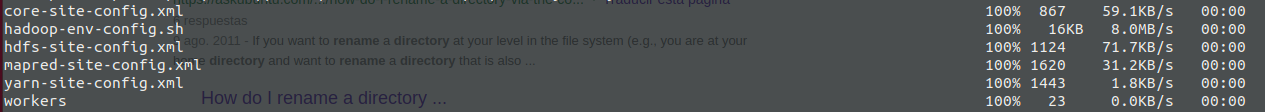
\includegraphics[width=.7\textwidth]{capitulo5/images/configuracionhadoopesclavo.png}
		\caption{Instalación de Hadoop en los nodos de datos/replica}
		\label{fig:pasarhadoop}
	\end{center}
\end{figure}
Una vez hecho esto, se procede a realizar la descompresión de los mismos y posteriormente a sobre escribir los archivos de configuración por defecto de Apache Hadoop por los archivos de configuración "Plantilla" recibidos del nodo maestro.\\
Con esto se terminaría el proceso de instalación y estaría todo listo para las tecnologías contempladas.\\
Al finalizar el instalador se deja a decisión y consideración del usuario realizar cambios sobre los archivos en caso de que requiera efectuar algún cambio antes de comenzar con su ambiente.\\
Cuando termine de hacer los cambios pertinentes, tendrá que ejecutar el siguiente comando en una terminal del nodo maestro con privilegios de super usuario:
\begin{verbatim}
hdfs namenode -format
\end{verbatim}
Lo que formateará toda la información contenida en el HDFS y con esto lo dejará disponible para ser utilizado como se puede ver en la figura \ref{fig:limpieza}.
\\
Es importante mencionar que esta tarea solo puede ser ejecutada una vez antes de comenzar el ambiente de Big Data. 
\begin{figure}[H]
	\hypertarget{fig:limpieza}{\hspace{1pt}}
	\begin{center}	
		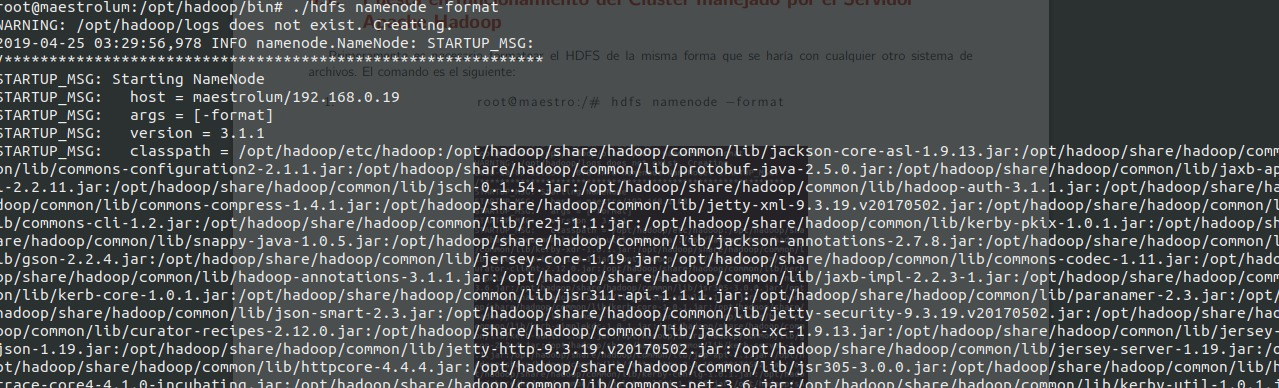
\includegraphics[width=.7\textwidth]{capitulo5/images/hadoop.jpeg}
		\caption{Limpieza del HDFS}
		\label{fig:limpieza}
	\end{center}
\end{figure}
Cuando el formateo esta terminado, entonces se procede a iniciar Apache Hadoop para que empiece su funcionamiento dentro de el ambiente distribuido, esto se puede hacer ejecutando el siguiente comando.
\begin{verbatim}
start-all.sh
\end{verbatim}
Con lo que comenzará a levantar e inicializar todas las dependencias necesarias para el funcionamiento de este framework como se puede ver en la figura \ref{fig:inicio}. 
\begin{figure}[H]
	\hypertarget{fig:inicio}{\hspace{1pt}}
	\begin{center}	
		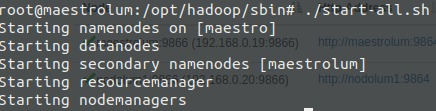
\includegraphics[width=.5\textwidth]{capitulo5/images/indice.jpeg}
		\caption{Inicio de Apache Hadoop}
		\label{fig:inicio}
	\end{center}
\end{figure}
Cuando se inicia Apache Hadoop en todos los nodos configurados mediante el instalador ya se puede acceder a su vista de configuración de esta herramienta desde la que se puede controlar su funcionalidad.
\\
Esto, se puede hacer accediendo a la dirección ip del nodo maestro en el puerto 9870 con el siguiente comando desde un navegador web :
\begin{verbatim}
[Direccion IP Maestro]:9870
\end{verbatim}
si se desea acceder a esta vista desde el propio nodo maestro se puede reemplazar la dirección ip con la instrucción de hacerlo en local host como se muestra a continuación:
\begin{verbatim}
localhost:9870
\end{verbatim}
La salida entonces para esta dirección web será como se muestra en la imagen \ref{fig:confi} donde podremos ver toda la configuración de todos los nodos en la red distribuida para Apache Hadoop. 

\begin{figure}[H]
	\hypertarget{fig:confi}{\hspace{1pt}}
	\begin{center}	
		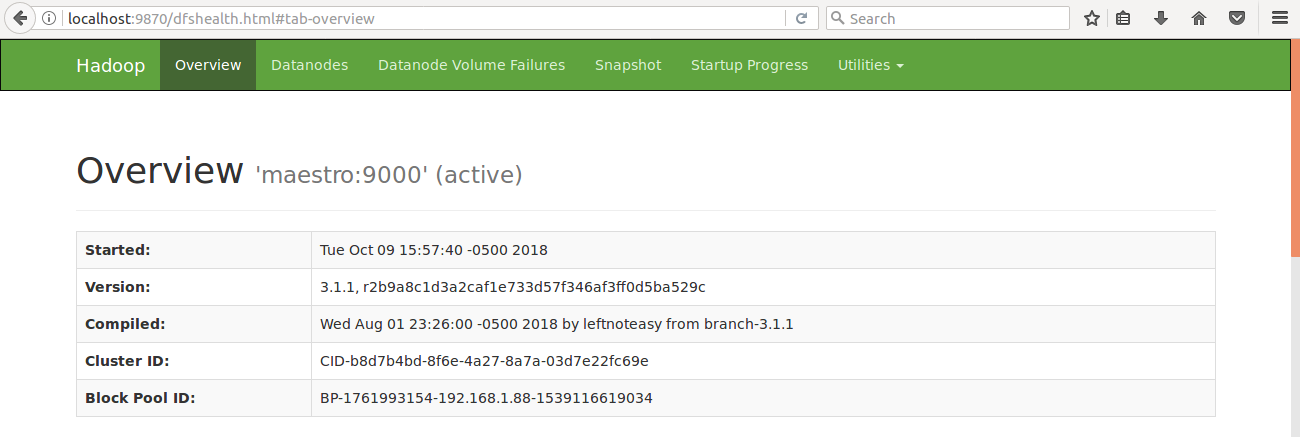
\includegraphics[width=.7\textwidth]{capitulo5/images/im54.png}
		\caption{Pantalla de configuración de Apache Hadoop}
		\label{fig:confi}
	\end{center}
\end{figure}
En este punto se da por terminado, las actividades y alcances del instalador, una vez terminado el paso 10 y comprobado que todo funciona correctamente, se puede afirmar que ya se tiene un ambiente de Big Data correctamente instalado y configurado ejecutándose en los equipos que forman parte de la red distribuida.


